\documentclass{standalone}

\usepackage{tikz}
\usetikzlibrary{fit,arrows, patterns, shapes.misc, positioning}

\tikzset{
    descr/.style={
        fill=white,
        inner sep=2.5pt
    },
    connector/.style={
     -latex,
     font=\normalsize
    },
    rectangle connector/.style={
        connector,
        to path={(\tikztostart) -- ++(#1,0pt) \tikztonodes |- (\tikztotarget) },
        pos=0.5
    },
    rectangle connectorh/.style={
        connector,
        to path={(\tikztostart) -- ++(0pt,#1)  -| (\tikztotarget) \tikztonodes },
        pos=0.5
    },
    rectangle connector/.default=-2cm,
    straight connector/.style={
        connector,
        to path=--(\tikztotarget) \tikztonodes
    }
}



\begin{document}


\resizebox{5.5cm}{!}{
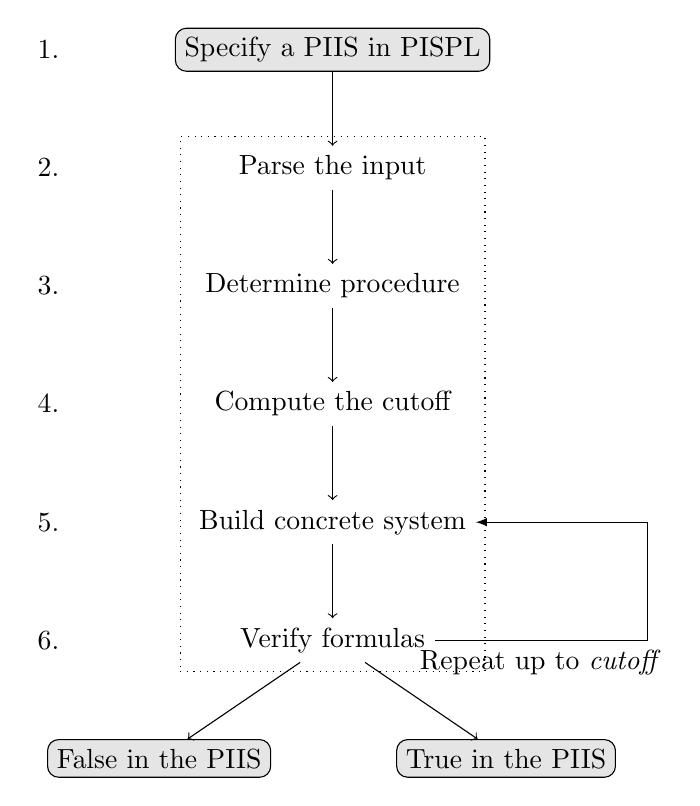
\begin{tikzpicture}[minimum width=1.5em,node distance=1.5cm, auto, s
node/.style={text width=11em,
           minimum height=1.5em,align=left}]

\node[] (s1) {$1.$};
\node[rectangle,draw=black,fill=black!10!white,rounded corners,right of=s1,xshift=6em] (1) {Specify a PIIS in PISPL};
\node[below of=s1] (s2) {$2.$};
\node[below of=1] (2) {Parse the input};
\node[below of=s2] (s3) {$3.$};
\node[below of=2] (3) {Determine procedure};
\node[below of=s3] (s4) {$4.$};
\node[below of=3] (4) {Compute the cutoff};
\node[below of=s4] (s5) {$5.$};
\node[below of = 4] (5) {Build concrete system};
\node[below of=s5] (s6) {$6.$};
\node[below of=5] (6) {Verify formulas};
\node[below of=6,rectangle,draw=black,fill=black!10!white,rounded corners, left
of=6,xshift=-2em] (7) {False in the PIIS};
\node[below of=6,rectangle,draw=black,rounded corners,fill=black!10!white,right
of=6,xshift=2em] (8) {True in the PIIS};



\path[->]
(1) edge (2)
(2) edge (3)
(3) edge (4)
(4) edge (5)
(5) edge (6)
(6) edge (7)
(6) edge (8);




\draw[->,rectangle connector=4cm] (6) to node[below] {Repeat up to
    $\it{cutoff}$} (5);

 \node[rectangle,draw=black,dotted,fit = (2) (3) (4) (5) (6) ] (x1) {};

%\draw[dotted, yshift=-18.5em] (0.75,1) rectangle (5.3,6);

%\node[s node] (template) {Template 
%  description in PISPL};
% \node[s node, inner sep=5pt,right=1cm of template]
% (spec) {Specification 
%  descriptions in PISPL};
%
% \node[s node, below=0.4cm of template] (parse) [xshift=4cm] {Parse Input};
% \node[s node, below=0.4cm of parse] (sim) {Simulation Test};
% \node[s node,below=0.4cm of sim] (cutoff) {Cutoff
% Identification};
% \node[s node,below =0.4cm of cutoff] (concrete) {Build BDDs
%   Encoding the Cutoff System};
%\node[s node,below=0.4cm of concrete] (verify) {Verify
%Formulas};
%\node[s node,below=0.4cm of verify,text width=7em] (true)
%[xshift=-4em] {True};
%\node[s node,below=0.4cm of verify,text width=7em] (false)
%[xshift=4em] 
%{False};
%   \path [line,font=\scriptsize] (template) edge
%                node  {} (parse);
%\path [line,font=\scriptsize] (spec) edge
%                node  {} (parse);
%\path [line,font=\scriptsize] (parse) edge
%                node  {} (sim);
%\path [line,font=\scriptsize] (sim) edge
%                node  {} (cutoff);
%\path [line,font=\scriptsize] (cutoff) edge
%                node  {} (concrete);
%\path [line,font=\scriptsize] (concrete) edge
%                node  {} (verify);
%\path [line,font=\scriptsize] (verify) edge
%                node  {} (true);
%\path [line,font=\scriptsize] (verify) edge
%                node  {} (false);
%

\end{tikzpicture}
}
\end{document}
